%
\documentclass[sigconf,review=false]{acmart}
\settopmatter{printacmref=false} % Removes citation information below abstract
\renewcommand\footnotetextcopyrightpermission[1]{} % removes footnote with conference information in first column
\pagestyle{plain} % removes running headers

\usepackage{pifont} % used for \todo symbol
\newcommand{\todo}[1]{
  %\textcolor{blue}{#1}
}
\newcommand{\note}[1]{
  \textcolor{red}{#1}
}
\usepackage{hyperref}
\usepackage{float}
\usepackage{soul}
\usepackage{booktabs}
\usepackage{multirow}

\newtheorem{definition}{Definition}

\def\BibTeX{{\rm B\kern-.05em{\sc i\kern-.025em b}\kern-.08emT\kern-.1667em\lower.7ex\hbox{E}\kern-.125emX}}
    
% Rights management information. 
% This information is sent to you when you complete the rights form.
% the commands and values with those provided to you when you complete the rights form.
%
% These commands are for a PROCEEDINGS abstract or paper.

% \copyrightyear{2018}
% \acmYear{2018}
% \setcopyright{acmlicensed}
% \acmConference[Woodstock '18]{Woodstock '18: ACM Symposium on Neural Gaze Detection}{June 03--05, 2018}{Woodstock, NY}
% \acmBooktitle{Woodstock '18: ACM Symposium on Neural Gaze Detection, June 03--05, 2018, Woodstock, NY}
% \acmPrice{15.00}
% \acmDOI{10.1145/1122445.1122456}
% \acmISBN{978-1-4503-9999-9/18/06}

%
% These commands are for a JOURNAL article.
%\setcopyright{acmcopyright}
%\acmJournal{TOG}
%\acmYear{2018}\acmVolume{37}\acmNumber{4}\acmArticle{111}\acmMonth{8}
%\acmDOI{10.1145/1122445.1122456}

%
% Submission ID. 
% Use this when submitting an article to a sponsored event. You'll receive a unique submission ID from the organizers
% of the event, and this ID should be used as the parameter to this command.
%\acmSubmissionID{123-A56-BU3}

%
% The majority of ACM publications use numbered citations and references. If you are preparing content for an event
% sponsored by ACM SIGGRAPH, you must use the "author year" style of citations and references. Uncommenting
% the next command will enable that style.
%\citestyle{acmauthoryear}

% The first command in your LaTeX source must be the \documentclass command.
%
% end of the preamble, start of the body of the document source.
\begin{document}

% These commands have SAMPLE values in them; it is your responsibility as an author to replace
%
% The "title" command has an optional parameter, allowing the author to define a "short title" to be used in page headers.
\title{Systematic Literature Review of Microservice Architectures}

%
% The "author" command and its associated commands are used to define the authors and their affiliations.
% Of note is the shared affiliation of the first two authors, and the "authornote" and "authornotemark" commands
% used to denote shared contribution to the research.

% \author{Ben Trovato}
% \authornote{Both authors contributed equally to this research.}
% \email{trovato@corporation.com}
% \orcid{1234-5678-9012}
% \author{G.K.M. Tobin}
% \authornotemark[1]
% \email{webmaster@marysville-ohio.com}
% \affiliation{%
%   \institution{Institute for Clarity in Documentation}
%   \streetaddress{P.O. Box 1212}
%   \city{Dublin}
%   \state{Ohio}
%   \postcode{43017-6221}
% }

\author{Thijmen J. Kurk}
\affiliation{%
  \institution{Vrije Universiteit Amsterdam, The Netherlands}
}
\email{t.j.kurk@student.vu.nl}


%
% By default, the full list of authors will be used in the page headers. Often, this list is too long, and will overlap
% other information printed in the page headers. This command allows the author to define a more concise list
% of authors' names for this purpose.
%\renewcommand{\shortauthors}{Verdecchia, et al.}

%
% The abstract is a short summary of the work to be presented in the article.
\begin{abstract}
  \todo{The abstract of the study goes here. A good abstract shortly summarizes the paper by covering: (i) a presentation of the topic covered, (ii) the research followed, (iii) the main findings of the study, and (iv) the outcome of the investigation}

  A microservice architecture is an interconnected web of small independent services that each run in its own process while interacting with each other using messages. These architectures are still evolving giving rise to the need for literature reviews. We aim at identifying and classifying definitions and patterns found in microservice architectures described by scientific literature into a concise model. Additionally, we set out to identify challenges found in inter-microservice data management and classify their possible solutions.
  Towards this goal, we apply well-known systematic literature review methods. Following these methods, we selected 21 relevant studies and iteratively updated our model based on these studies.
  This work contributes (i) a general model of a modern microservice architectures and (ii) an overview of challenges and solutions within inter-microservice data management.

\end{abstract}

%
% The code below is generated by the tool at http://dl.acm.org/ccs.cfm.
% Please copy and paste the code instead of the example below.
%
% \begin{CCSXML}
% <ccs2012>
%  <concept>
%   <concept_id>10010520.10010553.10010562</concept_id>
%   <concept_desc>Computer systems organization~Embedded systems</concept_desc>
%   <concept_significance>500</concept_significance>
%  </concept>
%  <concept>
%   <concept_id>10010520.10010575.10010755</concept_id>
%   <concept_desc>Computer systems organization~Redundancy</concept_desc>
%   <concept_significance>300</concept_significance>
%  </concept>
%  <concept>
%   <concept_id>10010520.10010553.10010554</concept_id>
%   <concept_desc>Computer systems organization~Robotics</concept_desc>
%   <concept_significance>100</concept_significance>
%  </concept>
%  <concept>
%   <concept_id>10003033.10003083.10003095</concept_id>
%   <concept_desc>Networks~Network reliability</concept_desc>
%   <concept_significance>100</concept_significance>
%  </concept>
% </ccs2012>
% \end{CCSXML}

% \ccsdesc[500]{Computer systems organization~Embedded systems}
% \ccsdesc[300]{Computer systems organization~Redundancy}
% \ccsdesc{Computer systems organization~Robotics}
% \ccsdesc[100]{Networks~Network reliability}

%
% Keywords. The author(s) should pick words that accurately describe the work being
% presented. Separate the keywords with commas.
\keywords{Systematic Literature Review, \todo{Other keywords identifying your study separated by comma} Microservice, Microservice Architecture, Data Management}

%
% A "teaser" image appears between the author and affiliation information and the body 
% of the document, and typically spans the page. 

%
% This command processes the author and affiliation and title information and builds
% the first part of the formatted document.
\maketitle

%\vspace{10pt}
\section{Introduction}
\todo{Present the topic of the literature review, including background of research field, goal, methodology, and contribution of the paper (e.g., map of the state of the art, reusable classification approach, evaluation of results, discussion of results, and target audience)}

Nowadays, microservices are the norm when software engineering scalable applications, especially considering that cloud computing and containerization technologies are becoming more prominent \cite{Jaramillo2016,Liu2020629,Akbulut201919}. Amazon, Netflix, LinkedIn, Spotify, SoundCloud and other companies \cite{7333476,Yahia20163, DiFrancesco201977} are actively adopting and evolving architectures in which microservices are deployed. The first definition of a microservice was introduced by \cite{martinfowler2014microservices} in 2014 as: \textit{'A service that can be automatically and independently be deployed, runs in its own process and communicates using lightweight mechanisms'}. Complementary to this definition, \cite{martinfowler2014microservices} specifies a microservice architecture (MSA) to be a collection of microservices working together towards desired business objectives.

The \textbf{goal} of this paper is to analyze published literature on MSAs and classify them. This classification will be done by iteratively creating a model using the definition of, and patterns in MSAs. Additional to this goal we zoom in on inter-microservice data management and classify problems and solutions commonly found therein.

The \textbf{audience} of this study are researchers, software engineers and developers who are interested in microservices or are inquisitive about the current state of inter-microservice data management.

The \textbf{outline} of this paper is as follows, Section~\ref{sec:related_work} discusses the relevant work we have found and how our research fits into this picture. Subsequently, Section~\ref{sec:design} goes into detail on how our systematic literature review is designed. Followed by Section~\ref{sec:results} where we define the model and answer our research questions based on the selected literature. Next, in Section~\ref{sec:discussion} we discuss the results. And finally in Section~\ref{sec:threats} and Section~\ref{sec:conclusion} we cover common threats to validity and conclude our study respectively.

To simplify to model used in Section~\ref{sec:results}, we choose to use the following definition of microservices (Definition~\ref{def:ms}) and MSAs (Definition~\ref{def:msa}) both originating from \cite{Garriga2018203}, where a process can be either be a process as defined by the operating system (OS) or a collection of threads within an OS process. These definitions generalize better and allow us to define a model that contains less edge cases. For example, using these definitions we can define services used for persistence to be microservices as well, although they do not directly implement logic towards any business objective. Additionally, we use the term service and microservice interchangeably in this paper.


\begin{definition}[Microservice, MS]\label{def:ms}
    A microservice is a cohesive independent process interacting via messages.
\end{definition}

\begin{definition}[Microservice Architecture, MSA]\label{def:msa}
    A microservice architecture is a distributed application where all its modules are microservices.
\end{definition}
\section{Related Work}
\label{sec:related_work}
\todo{Section dedicated to the related work, i.e., similar / relevant studies, and how your study fits in the overall research picture}

Numerous secondary studies on MSA have been performed \cite{Garriga2018203,Alshuqayran201644,Pahl2016137,Soldani2018215,Taibi2018221,DiFrancesco201977,Hamzehloui20191079}. A majority of these studies aim to provide an overview of what components generally reside in an MSA including but not limited to, how quality attributes \cite{o2007quality} can be applied to each of these components \cite{Garriga2018203, Alshuqayran201644, Pahl2016137}. Whereas others concentrate on the patterns in which these components can be utilized most effectively within MSAs \cite{Taibi2018221,richardson2018microservices, Akbulut201919,IBMBook,Messina2016223,5-newman2021building}.

This study distills the work published on MSAs into a model by iterating through studies systematically. In contrast to the work mentioned above, we put the focus on creating a general model of MSAs, instead of enumerating organizational aspects or specific patterns.



\section{Study Design}\label{sec:design}\label{sec:design}
% Section dedicated to document your study was carried out
This study is designed and carried out by following the guidelines on secondary studies \cite{syslit1,syslit2,syslit3}. We provide a replication package, which contains the raw data from each intermediate step executed during the search and selection phase (including any scripts that were used), over at our GitHub\footnote{\url{https://github.com/ThijmenKurk/literature-study}}.

\subsection{Research Approach}
\todo{What is the research goal of this study should be documented in this section. This can follow the GQM approach, as described in the following sentence, which NEEDS TO BE REPHRASED IN YOUR OWN WORDS if you want to include it in your study.}
\todo{In this subsection, the research questions underlying your study should be reported}

The goal of this literature study is to provide the reader with a model that contains an overview of components that are generally found inside microservice architectures. Furthermore, we describe the challenges and available solutions that are commonly used for the data management between microservices (i.e., transactions that spawn over multiple microservices). Towards our goal we have drafted the following research questions.
\begin{enumerate}
    \item[{RQ}1] How can modern microservice architectures be modelled?
    \item[    -] We drafted this research question to provide a generalizable model for modern microservice architectures derived from scientific literature. This high-level overview will facilitate the next research question by providing context, definitions, and concepts found in microservice architectures.
    \item[{RQ}2] What are the challenges and available solutions used for inter-microservice data management?
    \item[    -] We aim to identify challenges within inter-microservice data management such that we can expose the (potential lack of) available solutions.
\end{enumerate}

\subsection{Search and Selection}
\todo{How was the initial search for literature carried out should be reported in this section}
We now describe the search and selection process of this study. The study design (i.e., the search string and selection criteria) is locked in after the start of the search and selection process to avoid any personal biases. This and other threads to validity are discussed in Section \ref{sec:threats}.

\subsubsection{Initial Search}
For this study \textit{Elsevier Scopus}\footnote{\url{https://www.scopus.com/}} is used as our search engine. This tool has functionality such as the ability to, export search results to different formats (including but limited to CSV and BibTex), apply in-depth filters and search through both citations and references of studies automatically. All of which are used to facilitate the next steps. Our initial selection of 192 studies was a result of the query shown in Figure \ref{fig:search-string-refined}.


\begin{figure}
    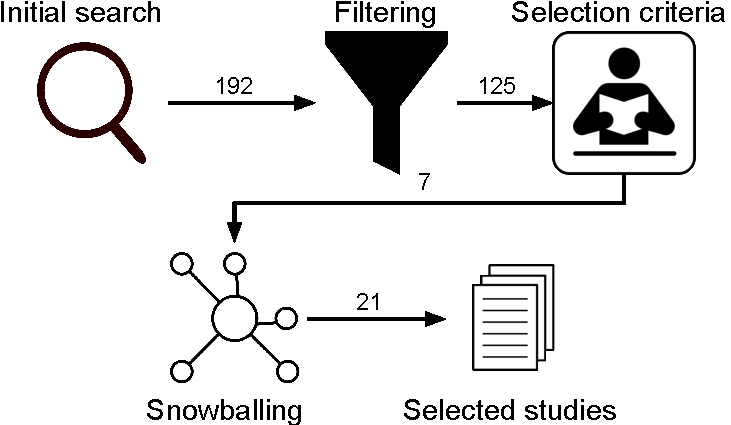
\includegraphics[scale=0.42]{images/search-and-selection.pdf}
    \caption{Search and selection process}
    \label{fig:search-and-selection}
\end{figure}

\subsubsection{Filtering}
Using the filter functionality of Scopus we were able to further refine our selection. First, all literature not pertaining to the subject area computer science is removed. Secondly, we filter the literature such that it only contains conference papers, articles and book chapters that are in a finalized state. Thirdly, we exclude any papers that are not written in English. Finally, we omit literature with the subject of microservices in combination with Internet of Things (IoT) and network architectures, since this is out of scope of this review. Refining our selection to a total of 125 studies.


\subsubsection{Application of Selection Criteria}
\todo{ In this section, the selection criteria, in terms of inclusion and inclusion criteria should be documented. See examples below, which should be adapted to your specific case and, in any case, *rephrased in our own words*}

The selected studies are manually filtered using the inclusion and exclusion criteria \cite{syslit1,syslit2,syslit3} listed below.
\begin{enumerate}
    \item[{I}1] Studies focussing on microservices or microservice architectures.
    \item[{I}2] Studies focussing on data management within microservice architectures.
    \item[{I}3] Studies that are peer-reviewed.
    \item[{I}4] Studies that are written in English.
    \item[{E}1] Studies that marginally describe a microservice architecture.
    \item[{E}2] Studies describing the migration process from a monolith to microservice architecture.
    \item[{E}3] Studies that are of bad quality (e.g., many spelling errors, unreadable sentences, etc.)
    \item[{E}4] Studies not available as full-text.
\end{enumerate}
\begin{equation}
    (I1 \vee I2) \wedge I3 \wedge I4 \wedge \neg E1  \wedge \neg E2  \wedge \neg E3  \wedge \neg E4
    \label{eq:inc_excl_criteria}
\end{equation}

The criteria are applied by following equation~\ref{eq:inc_excl_criteria} during each of the following two steps. First, we read the title and abstract of the study. Last, we read each study full-text. After the manual filtering is done we are left with a selection of 7 studies.

\subsubsection{Snowballing}
\todo{If a snowballing approach was used for the literature review, its details should be documented in this subsection}
During this phase \textit{forward} and \textit{backward} snowballing \cite{syslit4} is used on the selected studies. On completion, we expanded our selection to 21 studies.

\subsubsection{Final Selection}
The search and selection process selected 21 studies for this review. An overview of the selected studies can be found in Table~\ref{table:selected-studies}.

% \subsubsection{Exclusion during Data Extraction}
% \todo{Write about studies excluded after being read for a second time in the Data Extraction phase}

\subsection{Data Extraction}
\todo{Report in this section the data extraction followed to gather the data for the study (e.g., what process did you followed to gather the data in the companion data extraction spreadsheet?)}
During the data extraction phase, every selected study is read full-text and information pertaining to the research questions is stored in a spreadsheet. The goal of this phase it to find patterns within MSAs such that the primary components within these patterns can be described and modelled.

\subsection{Data Synthesis}
During the data synthesis phase we iteratively go through the extracted data and update our model to fit it. This method is called narrative synthesis and is commonly used when synthesizing literature in the context of systematic literature reviews \cite{popay2006guidance}. The product of this step is a generalized model of MSAs and the challenges and potential solutions within data management, both of which are described in Section~\ref{sec:results}.


% \subsection{Study Replicability}
% \todo{To ensure the replicability of the study, you should document in this section the data you make available (e.g. via Google Drive) to replicate the findings, this include:
%     * the research protocol
%     * the complete list of primary studies
%     * the parameters composing the potential classification framework you built
%     * the raw extracted data of each selection phase}

\begin{figure*}[tpb]
    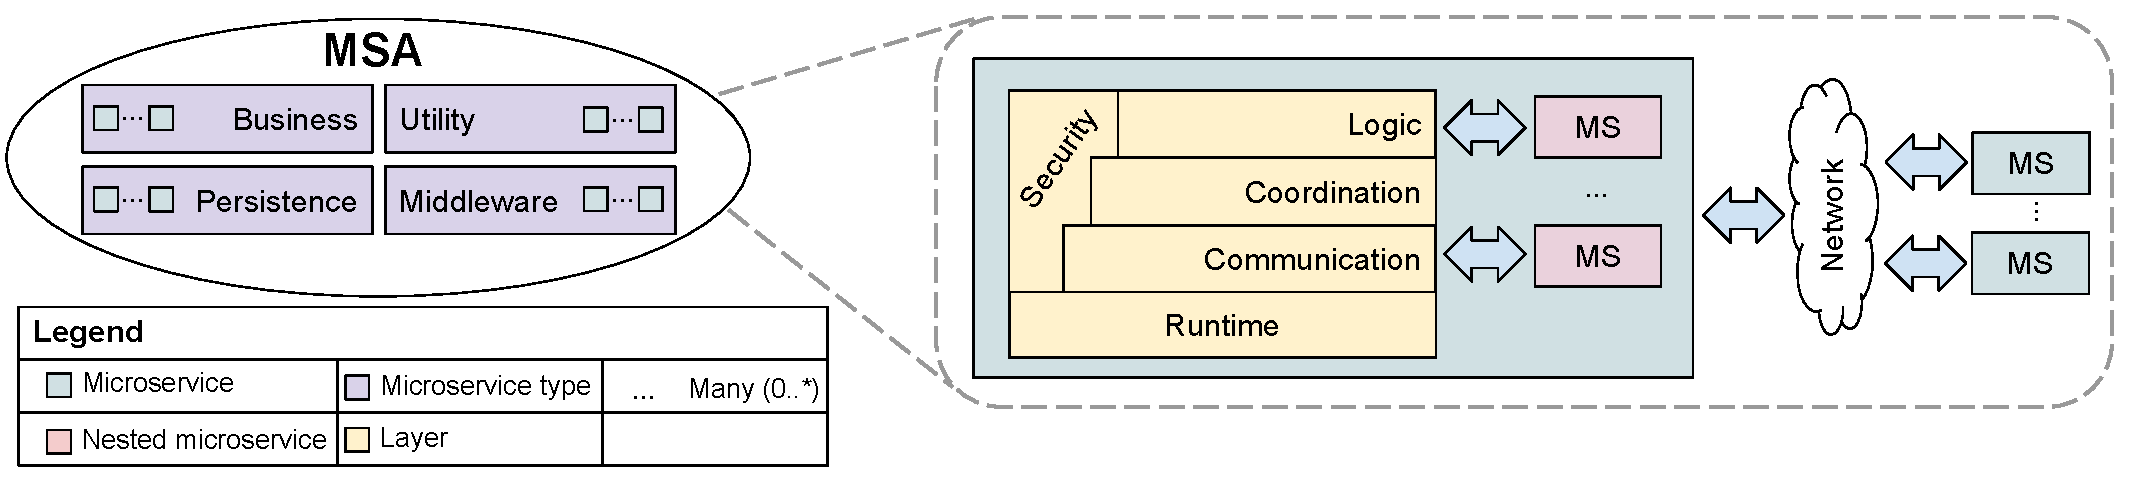
\includegraphics[scale=0.42]{images/msa-model.pdf}
    \caption{Generalized model of microservice architectures}
    \label{fig:model}
\end{figure*}

\section{Results}\label{sec:results}
\todo{In this section, the results of the literature review should be reported. This section can be split up according to the specific focus of the literature review, e.g. Publication Trends, Research Focus, and Potential for Industrial Adoption (see Running example)}

In this section we discuss the results of our literature review. The iterative model created from the selected studies is displayed in Figure~\ref{fig:model}. It defines the main components inside a microservice on an implementation level without detailing any topological specifics. Now the model is described.

\subsection{The Model}

There are four types of microservices, all of which are interconnected with other microservices through a network. (i) Business microservices implement logic towards a business objective, (ii) utility microservices facilitate business microservices with general functionality (e.g., logging, monitoring, circuit breakers, load balancers, service discovery, etc. \cite{richardson2018microservices}), (iii) persistence microservices typically provide database management systems (DBMS) or cache systems to business microservices, and finally (iv) middleware services which facilitate communication between other microservices (e.g., an API gateway, a message broker, a message bus, etc. \cite{richardson2018microservices,Garriga2018203}). An MSA is an interdependent cohesive loosely-coupled composition of these four types of services.

Every microservice can have nested microservices which only the parent microservice is allowed to communicate with. Nested microservices can be colocated on the same node as the parent microservice or hosted on separate nodes \cite{richardson2018microservices}. The former is generally the case with the sidecar pattern in which nested utility microservices are deployed to abstract away general functionality from the parent, while the latter is often the case with persistence services \cite{5-newman2021building,richardson2018microservices}.
A microservice consists of 3 layers with one overarching layer being security \cite{Garriga2018203,richardson2018microservices,Sill201676,5-newman2021building} and one foundational layer being runtime. Each layer is now described.

\textbf{Runtime} of a microservice consists of the platform on which it is executed. The industry has evolved such that physical hardware is abstracted away behind many layers of virtualization \cite{richardson2018microservices}. There are two levels of virtualization relevant to MSAs, (i) Hardware Abstraction Layer (HAL) virtualization (i.e., virtual machines \cite{richardson2018microservices}) and (ii) OS-level virtualization (i.e., containers \cite{Jaramillo2016,richardson2018microservices}). Microservices are typically deployed in either, or a combination, of these types of virtualized environment \cite{DiFrancesco201977}.

\textbf{Communication} between microservices consists of three parts \cite{Sill201676}, (i) the interaction model, (ii) the transportation and finally (iii) the presentation. The interaction model between services can be synchronous or asynchronous. Synchronous communication implies a request/response type pattern, meaning that it is vulnerable for services blocking other services while they are waiting for a response \cite{5-newman2021building, richardson2018microservices, IBMBook}. Asynchronous communication is non-blocking by definition and often comes hand in hand with event-based architectures \cite{Unlu2021244}. However, it requires state management within microservices and typically incurs more communication overhead due to it generally requiring some kind of middleware service, such as a message broker or message bus to facilitate and decouple message delivery \cite{richardson2018microservices, middleware, IBMBook}. Messages between microservices are transported either via the network or through Inter Process Communication (IPC) depending on performance and scalability requirements. The protocol used for transportation should be selected while considering the desired interaction model, since it can be performed using a variety of protocols \cite{Sill201676} (e.g., HTTP, gRPC, XMPP, MQTT, AMQP, etc.). Finally, presentation describes how the data is serialized such that it can be transported between services. Common serializers are JSON, XML and Protobuf \cite{richardson2018microservices}.

\textbf{Coordination} between services inside an MSA is necessary since it is a distributed system per definition \cite{5-newman2021building,richardson2018microservices, IBMBook}. The coordination within an MSA to perform more complex and elaborate functionalities are either choreography or orchestration based \cite{Garriga2018203,richardson2018microservices,4196179}. Orchestration requires composite services that directly coordinates with other services to oversee the process by receiving responses. On the other hand, choreography uses asynchronous events with the publish/subscribe pattern to facilitate collaboration \cite{Garriga2018203,richardson2018microservices,5-newman2021building}.

In essence, the coordination between microservices is about data management \cite{Laigner20213348}. There are  various challenges in data management all of which are subject of the next research question.

\textbf{Logic} is the last layer inside of microservices and includes all the programming required to implement the necessary functionality for each particular service. This can be anything due to our wide definition of microservices, ranging from business logic to DBMS logic. One important part of the logic layer is state management. Service can either be stateful or stateless \cite{IBMBook}. Statefulness implies session affinity, which in term means less flexibility and scalability \cite{7937885}. How and if state should be managed within a service can therefore be determined from the scalability requirements of that service.

\textbf{Security} is a layer that overarches all the previously defined layers and is challenging to implement properly. However, it vital within MSAs, due to the large attack surface and complicated connections between services \cite{shmeleva2020microservices}. There are two approaches to securing distributed systems, either a zero-trust-network or a trust-the-network approach \cite{christudas2019microservices,barth2017zero}. Depending on the security requirements of the MSA, a certain network type should be chosen \cite{shmeleva2020microservices,christudas2019microservices,Garriga2018203,barth2017zero}.

\subsection{Data Management}
The functionality of business microservices is commonly determined by applying domain-driven design (DDD) techniques \cite{evans2004domain}. In DDD, the problem space of the business is referred to as the domain. This domain can be divided into multiple subdomains each representing a different part of the business. Every subdomain has its own domain model, the scope of which is called a bounded context \cite{richardson2018microservices,Dragoni2017195,Unlu2021244,Santos2019145}. From this bounded context, one or more business microservices can be derived \cite{richardson2018microservices}. Typically, there is some (minimal) data dependency between the bounded context of these services. Therefore, inter-microservice data management (handled by the coordination layer in the model, Figure~\ref{fig:model}) is required, given that MSAs are commonly designed with a database per service pattern \cite{Soldani2018215}. According to the \textbf{CAP} theorem, any networked system which shares \textbf{P}artitions of data can only pick one of/attain a balance between the following two properties: \textbf{A}vailability or \textbf{C}onsistency \cite{6133253}. For example, a highly available MSA cannot be consistent all the time \cite{richardson2018microservices}. Therefore, depending on the consistency and availability requirements of the MSA, different solutions to facilitate inter-microservice data management are desirable. We now describe three common data management challenges found within MSAs.

\subsubsection{Inter-microservice data relations}\label{sec:foreign}
Consider two business microservices, one that keeps track of departments and one that keeps track of employees. Every department can have zero-to-many employees. In a relational DBMS, this type of relation is enforced by a foreign key on employee referring to the department of which the employee is a part of. The DBMS enforces policies to keep the database consistent, by for example, cascade deleting employees that are member of a deleted department, or making sure that every employee is member of a valid department. However, this type of enforcement is not trivial if each service has its own (possibly different type of) DBMS \cite{richardson2018microservices,5-newman2021building, Laigner20213348}. Foreign key emulation is currently resolved using ad-hoc implementations due to the lack of a general solution \cite{Laigner20213348}.

\subsubsection{Inter-microservice data transactions}
A transaction is a unit of work that needs to be completed in its entirety or rolled back. This is challenging to implement in MSAs due to the use of (polyglot) distributed persistence \cite{richardson2018microservices,IBMBook,Laigner20213348}. Consider two business microservices, $X_1$ that keeps track of inventory and $X_2$ that is responsible for the placement and tracking of orders. When an order is placed, the stock of the product is updated through the inventory service. A product with only one left in the stock is ordered by two users at the same time. Now $X_2$ receives two requests to check the stock followed by two requests to update the stock. A naive implementation allows the product to be ordered twice, since $X_1$ and $X_2$ do not coordinate the transaction. There are two solutions for this problem, depending on the desired properties of the MSA, displayed in Table~\ref{table:transactions}.

\textbf{Saga} is pattern in which eventual data consistency can be guaranteed by splitting up inter-microservice transactions into a sequence of compensable (potentially retryable) subtransactions each having the scope of only a single microservice \cite{richardson2018microservices,Laigner20213348}. A Saga transaction is successful if each subtransaction has succeeded and can be coordinated using either a choreography or an orchestration based interaction model \cite{richardson2018microservices}. If one subtransaction fails, the already succeeded subtransactions are rolled back by executing their respective compensating subtransactions. This makes the MSA eventual consistency and basically available \cite{6133253}.

\textbf{Two-Phase Commit (2PC)} is a pattern in which strong data consistency is guaranteed by orchestrating each operation of the inter-microservice transaction in two phases \cite{Laigner20213348,richardson2018microservices}. The transaction orchestrator starts the first phase by requesting each service to prepare the necessary operations and waiting for each to respond. The second phase executes after each service has successfully prepared and makes the operations permanent. The first phase requires each service to lock resources until the transaction is finalized or aborted since otherwise transactional consistency cannot be guaranteed \cite{ports2010transactional,Laigner20213348}. This trades availability for strong data consistency \cite{richardson2018microservices}.

\begin{table}
    \begin{tabular}{p{1.5cm}p{2cm}p{2cm}l}
        \toprule
        \textbf{Pattern}       & \textbf{Interaction Model}       & \textbf{Consistency}                     & \textbf{Availability}              \\
        \midrule
        \multirow{2}{*}{Sagas} & Orchestration,                   & \multirow{2}{2cm}{Eventually consistent} & \multirow{2}{*}{Available}         \\
                               & Choreography                     &                                          &                                    \\
        \hline
        Two-Phase              & \multirow{2}{2cm}{Orchestration} & \multirow{2}{2cm}{Consistent}            & \multirow{2}{2cm}{Less available } \\
        Commit                 &                                  &                                          &                                    \\
        \bottomrule
    \end{tabular}
    \caption{Inter-microservice transaction patterns}
    \label{table:transactions}
\end{table}

\subsubsection{Inter-microservice query aggregation and joining}
When a microservice requires data from multiple service, it needs to retrieve and aggregate data from each microservice individually and deal with possible inconsistencies by itself \cite{Laigner20213348}. These inconsistencies can form due to, for example, the incorrect implementation of ad-hoc solutions described in Section~\ref{sec:foreign} or a service failing to return the requested data \cite{richardson2018microservices}. Typically, queries that require aggregation or joins are highly optimized inside of DBMSs. Therefore, performing them manually on data from different services implies steep performance penalties. A common solution to this problem is the Command Query Responsibility Segregation (CQRS) pattern. With CRQS, so-called views (read only copies) of tables are prematurely colocated at microservices that require them to speed up aggregation and join operations \cite{richardson2018microservices}. Only the microservice owning the table can write to it. Writes are streamed to the views via events using the publish/subscribe pattern, making them eventually consistent \cite{richardson2018microservices}.
















\section{Discussion}\label{sec:discussion}
\todo{In this section, the results of the literature review should be reported. This section can be split up according to the specific focus of the literature review, e.g. Publication Trends, Research Focus, and Potential for Industrial Adoption (see Running example)}
This literature review aimed to model modern MSAs and the important components within them. This provides researchers with an overview of important aspects and layers to consider while implementing MSAs. We found similar studies within our selection of literature, but these studies considered different aspects of MSAs (e.g., organizational aspects or architectural aspects) instead of implementation aspects.

Additionally, this study derived three challenges and potential solutions for data management problems within MSAs from the selected literature. The lack of solutions for some of these challenges show that MSAs are still evolving and not fully mature yet.
\section{Threats to Validity}\label{sec:threats}
\todo{In this section, the most prominent threats to validity of your study should be discussed.}
In this section, we discuss the most prominent threats to validity of this study.

\textbf{Internal validity.}
The internal validity threat is related to the design and execution of the literature review \cite{syslit3}. This threat is mitigated by defining a detailed research protocol in Section~\ref{sec:design} and locking this protocol so that it cannot change after the review is started to prevent personal bias.

\textbf{External validity.}
The external validity threat is related to the generalizability of the results \cite{syslit3}. More specifically, for a literature study this would mean that the selected studies not being representative of the full population (i.e., all the available published literature). To mitigate this form of bias, we used a generic search query (Figure~\ref{fig:search-string-refined}) inside of a search engine that indexes scientific literature from multiple sources. Additionally, we utilized both forward and backward snowballing \cite{syslit4} to further expand our selected literature with studies our automatic search might have missed.


\textbf{Construct validity.}
The construct validity threat concerns the relation between theory and observation. We mitigated this bias by searching multiple sources using Scopus with only general terms in our search string. Additionally, we rigorously selected relevant studies according to inclusion and exclusion criteria \cite{syslit1,syslit2,syslit3}.

\textbf{Conclusion validity.}
The conclusion validity concerns the degree in which our conclusions are reasonable based on our extracted data. We mitigated this by iteratively defining and updating our model during the data extraction and synthesis phase. Additionally, this threat was mitigated by applying well-known systematic literature review methods \cite{syslit1,syslit2, syslit3, syslit4}.
\section{Conclusion}\label{sec:conclusion}
\todo{Conclusion of your investigation, including (i) few sentence to introduce the topic considered, (ii) short summary of the research method followed, (iii) main findings, and (iv) potential implications and future work}
This study gives an overview of modern microservice architectures in the form of a model and identified three data management challenges and their potential solutions by systematically analyzing the latest studies on microservices using well-known literature review methods \cite{syslit1, syslit2,syslit3,syslit4}.

We found that microservices consist of four layers: (i) Runtime, (ii) Communication, (iii) Coordination and (iv) Logic, with one overarching layer being Security. These microservices are connected with each other to form a microservice architecture. There are four types of microservices: (i) Business, (ii) Utility, (iii) Persistence and (iv) Middleware. Additionally, we found three data management challenges: (i) inter-microservice data relations, (ii) inter-microservice data transactions and (iii) inter-microservice query aggregation and joining. We conclude that microservice architectures are evolving but that they are far from mature, given the fact that not all data management challenges have general solutions.

In the future we would like to explore how to solve the challenge described in Section~\ref{sec:foreign} by proposing a general solution for this problem.



\bibliographystyle{ACM-Reference-Format}
\bibliography{bibliography}


\begin{figure}
    \ul{\texttt{TITLE("microservice?") AND (TITLE("architecture") OR (TITLE("data") AND (TITLE("coordination") OR TITLE("management"))))}} \texttt{ AND (LIMIT-TO(PUBSTAGE, "final")) AND (LIMIT-TO(DOCTYPE, "cp") OR LIMIT-TO(DOCTYPE, "ar") OR LIMIT-TO(DOCTYPE, "ch")) AND (LIMIT-TO(SUBJAREA, "COMP")) AND (LIMIT-TO(LANGUAGE, "English")) AND (EXCLUDE(EXACTKEYWORD, "Internet Of Things") OR EXCLUDE(EXACTKEYWORD, "Network Architecture"))}
    \caption{\ul{The initial search string} and the refined search string after the filtering process}
    \label{fig:search-string-refined}
\end{figure}


\begin{table*}[!t]
    \begin{tabular}{llp{3in}p{2in}r}
        \toprule
        {} & \textbf{Document Type} & \textbf{Title}                                                                                      & \textbf{Authors}                                                                                    & \textbf{Year} \\
        \midrule
        1  & Article                & Performance Analysis of Choreography and Orchestration in Microservices Architecture                & Kristianto, H., Zahra, A.                                                                           & 2021          \\
        2  & Conference Paper       & Data management in microservices: State of the practice, challenges, and research directions        & Laigner, R., Zhou, Y., Salles, M.A.V., Liu, Y., Kalinowski, M.                                      & 2021          \\
        3  & Conference Paper       & Microservices: Architecture, container, and challenges                                              & Liu, G., Huang, B., Liang, Z., Qin, M., Zhou, H., Li, Z.                                            & 2020          \\
        4  & Conference Paper       & A logical architecture design method for microservices architectures                                & Santos, N., Salgado, C.E., Morais, F., Melo, M., Silva, S., Martins, R., Pereira, M., Rodrigues,... & 2019          \\
        5  & Conference Paper       & A Comparative Review of Microservices and Monolithic Architectures                                  & Al-Debagy, O., Martinek, P.                                                                         & 2018          \\
        6  & Conference Paper       & Towards a taxonomy of microservices architectures                                                   & Garriga, M.                                                                                         & 2018          \\
        7  & Conference Paper       & Leveraging microservices architecture by using Docker technology                                    & Jaramillo, D., Nguyen, D.V., Smart, R.                                                              & 2016          \\
        8  & Conference Paper       & A systematic mapping study in microservice architecture                                             & Alshuqayran, N., Ali, N., Evans, R.                                                                 & 2016          \\
        9  & Conference Paper       & Microservices: A systematic mapping study                                                           & Pahl, C., Jamshidi, P.                                                                              & 2016          \\
        10 & Article                & The pains and gains of microservices: A Systematic grey literature review                           & Soldani, J., Tamburri, D.A., Van Den Heuvel, W.-J.                                                  & 2018          \\
        11 & Article                & Microservices Patterns                                                                              & Richardson, C.                                                                                      & 2018          \\
        12 & Article                & Microservices: Yesterday, today, and tomorrow                                                       & Dragoni, N., Giallorenzo, S., Lafuente, A.L., Mazzara, M., Montesi, F., Mustafin, R., Safina, L.    & 2016          \\
        13 & Conference Paper       & Architectural patterns for microservices: A systematic mapping study                                & Taibi, D., Lenarduzzi, V., Pahl, C.                                                                 & 2018          \\
        14 & Article                & The Design and Architecture of Microservices                                                        & Sill, A.                                                                                            & 2016          \\
        15 & Conference Paper       & The database-is-the-service pattern for microservice architectures                                  & Messina, A., Rizzo, R., Storniolo, P., Tripiciano, M., Urso, A.                                     & 2016          \\
        16 & Article                & Performance Analysis of Microservice Design Patterns                                                & Akbulut, A., Perros, H.G.                                                                           & 2019          \\
        17 & Conference Paper       & Microservices architecture: Challenges and proposed conceptual design                               & Munaf, R.M., Ahmed, J., Khakwani, F., Rana, T.                                                      & 2019          \\
        18 & Article                & Microservices from theory to practices                                                              & Daya, S.                                                                                            & 2015          \\
        19 & Conference Paper       & Event Oriented vs Object Oriented Analysis for Microservice Architecture: An Exploratory Case Study & Unlu, H., Tenekeci, S., Yildiz, A., Demirors, O.                                                    & 2021          \\
        20 & Article                & Architecting with microservices: A systematic mapping study                                         & Di Francesco, P., Lago, P., Malavolta, I.                                                           & 2019          \\
        21 & Conference Paper       & A systematic mapping study on microservices                                                         & Hamzehloui, M.S., Sahibuddin, S., Salah, K.                                                         & 2019          \\
        \bottomrule
    \end{tabular}
    \caption{Selected studies}
    \label{table:selected-studies}
\end{table*}

% 
% If your work has an appendix, this is the place to put it.
%\appendix


\end{document}
